\documentclass[12pt]{article}
\usepackage{amsmath,amsfonts, epsfig}
\usepackage{booktabs} % for better table formatting
\usepackage[authoryear]{natbib}
\usepackage{array}
\usepackage{multirow}
\usepackage{graphicx}
\usepackage{fancyhdr}
\usepackage{bm}
\pagestyle{fancy}
\lfoot{\texttt{ematm0067.github.io} / \texttt{ematm0044.github.io}}
\lhead{Introduction to AI - 02.4\_logistic - Conor}
\rhead{\thepage}
\cfoot{}

\usepackage{tikz}
\usetikzlibrary{positioning}

\usepackage{ifthen}
\newboolean{nopics}
\setboolean{nopics}{true}


\begin{document}

\section*{Logistic regression.} 

Lets begin with an example, the Canadian linguist Jack Chambers is
interested in dialect and language change among English speakers in
the eastern part of Canada. He did a broad study where he discovered
many on-going changes and tried to interpret them. The data are
available, at least in summary form at
\texttt{dialect.topography.artsci.utoronto.ca/}. In one example, from
what is called the Golden Horseshoe, which extends along the western
shore of Lake Ontario and includes the cities of Hamilton and Toronto,
he discovered what to me looks like a surprising shift from weak to
strong participle for the word \textsl{sneak}. He asked participants which they say from
\begin{itemize}
\item The little devil sneaked into the theatre.
\item The little devil snuck into the theatre.
\end{itemize}
and roughly speaking found that younger people prefer `snuck' to
`sneaked', the so called strong form over the weak. I had assumed
there was a general trend towards weak forms.

This graph below gives a simulated version of his data; the actual
data have more points but bundle the participants into age bands. For
the convenience of this lesson I have made artificial data, with fewer
points but where the ages take any whole-year value: the artificial
data is designed to have the same broad statistical structure as the
real data. In the graph age is plotted along the bottom, and the
$y$-value is zero for participants who say they use `snuck' and one
for those who use `sneaked'. A small jitter has been added to the $y$
value to stop the points covering each other, this is a common and
useful graphical device used for data like this.
\begin{center}
  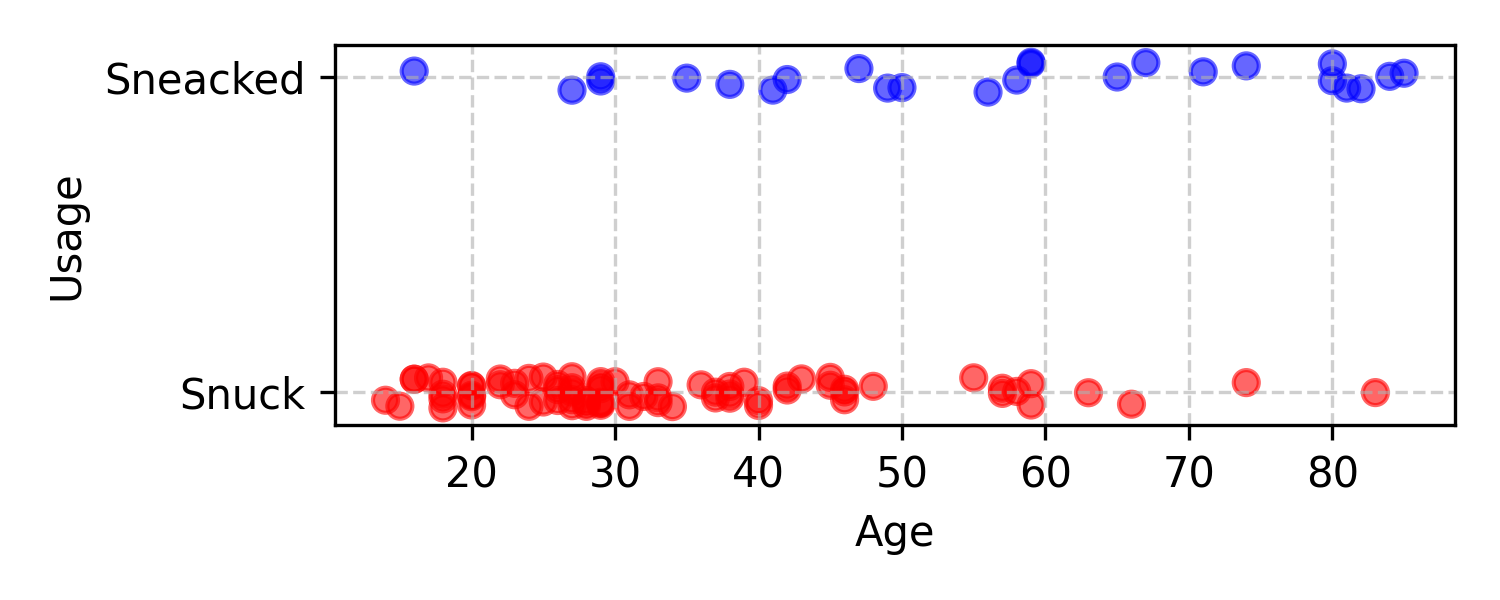
\includegraphics[]{02.4_sneak.png}
  \end{center}
  Now, clearly there is something going on. If we take these data and
  bin them in ten year age bands and calculating for each band what
  fraction for each band says `sneaked' we get this:
\begin{center}
  \includegraphics[]{02.4_proportion.png}
  \end{center}
  and it is obvious that younger people say `snuck' more often than
  older. However, what we have learned so far is to model
\begin{equation}
\hat{u}=\beta_1 a+\beta_0
\end{equation}
where $a$ is the age and $u$ is some measure of
`snuck-saying-ness'. This, though, clearly does not work.

\section*{Summary}
In linear regression we assume the data come from a noisy version of a
linear process and we seek to model that process. It turns out there
is an analytic formula for the model parameters. This generalizes to
linear models that have lots of inputs and lots of predictions. The
error associated with the model can be minimimized by gradient flow,
since this is a solved problem it seems weird to do it approximately,
however numerical approaches like gradient descent works in other
cases where there is no analytic solution. We see how gradient on our
simple example.
\end{document}

